\section{Auswertung}

\subsection{Einzelspalt \label{sec:ein}}

In Tabelle \ref{tab:ein} befinden sich die aufgenommenen Messwerte.
\begin{table}[H]
   \centering
   \caption{Aufgenommene Messwerte zur Bestimmung der Breite des Einzelspalts} 
   \label{tab:ein}
   \begin{tabular}[t]{ c c }
 \toprule
 {$x\:/\: \mathrm{mm}$} & {$I\:/\: \mathrm{μA}$} \\
    \midrule
    10,0 & 0,0055 \\
    10,5 & 0,0065 \\
    11,0 & 0,0085 \\
    11,5 & 0,0110 \\
    12,0 & 0,0135 \\
    12,5 & 0,0165 \\
    13,0 & 0,0190 \\
    13,5 & 0,0205 \\
    14,0 & 0,0210 \\
    14,5 & 0,0205 \\
    15,0 & 0,0185 \\
    15,5 & 0,0160 \\
    16,0 & 0,0130 \\
    16,5 & 0,0100 \\
    17,0 & 0,0085 \\
    17,5 & 0,0095 \\
    18,0 & 0,0130 \\
    18,5 & 0,0200 \\
    19,0 & 0,0300 \\
    19,5 & 0,0480 \\
    20,0 & 0,0700 \\
    20,5 & 0,0900 \\
    21,0 & 0,1250 \\
    21,5 & 0,1550 \\
    22,0 & 0,1950 \\
    22,5 & 0,2250 \\
    23,0 & 0,2600 \\
    23,5 & 0,2600 \\
    24,0 & 0,2900 \\
    24,5 & 0,3000 \\
    25,0 & 0,3200 \\
    25,5 & 0,3000 \\
    26,0 & 0,3000 \\
    \bottomrule
  \end{tabular}
    \qquad
  \begin{tabular}[t]{c c}
    \toprule
    {$x\:/\: \mathrm{mm}$} & {$I\:/\: \mathrm{μA}$} \\
    \midrule
    26,5 & 0,2800 \\
    27,0 & 0,2600 \\
    27,5 & 0,2400 \\
    28,0 & 0,2000 \\
    28,5 & 0,1800 \\
    29,0 & 0,1300 \\
    29,5 & 0,1000 \\
    30,0 & 0,0850 \\
    30,5 & 0,0680 \\
    31,0 & 0,0440 \\
    31,5 & 0,0280 \\
    32,0 & 0,0160 \\
    32,5 & 0,0115 \\
    33,0 & 0,0075 \\
    33,5 & 0,0060 \\
    34,0 & 0,0085 \\
    34,5 & 0,0110 \\
    35,0 & 0,0135 \\
    35,5 & 0,0160 \\
    36,0 & 0,0175 \\
    36,5 & 0,0180 \\
    37,0 & 0,0180 \\
    37,5 & 0,0170 \\
    38,0 & 0,0150 \\
    38,5 & 0,0130 \\
    39,0 & 0,0105 \\
    39,5 & 0,0085 \\
    40,0 & 0,0065 \\
    40,5 & 0,0055 \\
    41,0 & 0,0045 \\
    41,5 & 0,0045 \\
    42,0 & 0,0045 \\
    \bottomrule
  \end{tabular}
\end{table}


Von der Intensität $I$ muss noch der Dunkelstrom $I_\text{d} = \SI{0,002}{} \: \symup{μA}$ abgezogen werden. Im Anschluss werden diese normiert.
Diese Werte sind in Abbildung \ref{fig:ein} aufgetragen.
\begin{figure}[H]
  \centering
  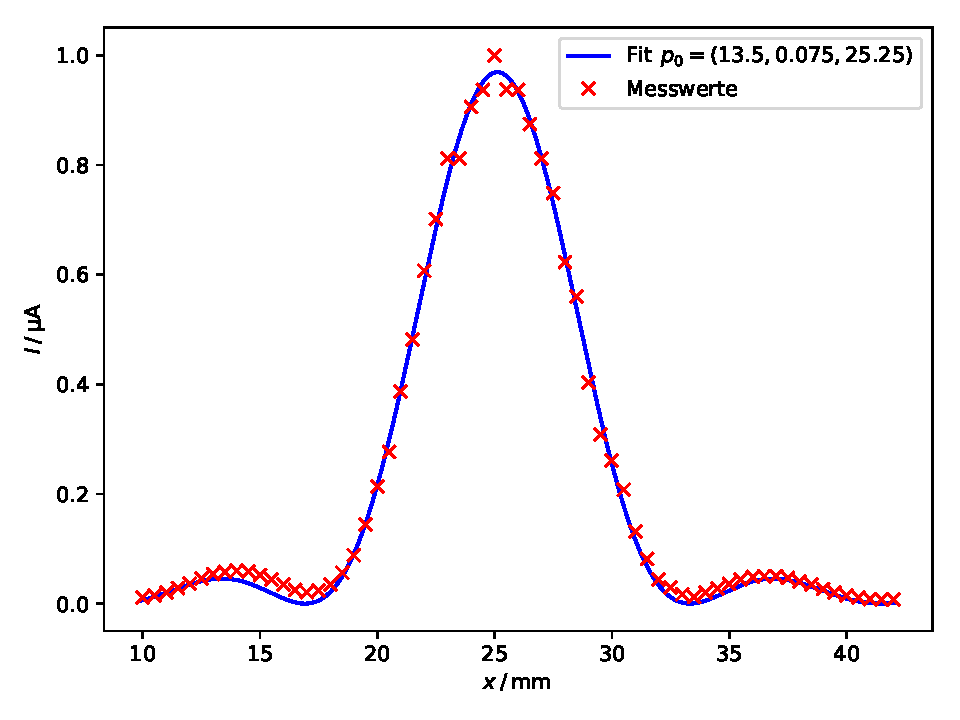
\includegraphics[width=\textwidth]{Plots/einzel.pdf}
  \caption{Graph zur Bestimmung der Breite des Einzelspalts mit den Parametern $(A_0, b, x_0)$.}
  \label{fig:ein}
\end{figure}

Eine Regression
\begin{equation*}
  f(x) = A^2_0 b^2 \left(\frac{\lambda}{\pi b \sin{\!\left(\frac{x-x_0}{L} \right)}}\right)^2 \sin^2{\!\left(\frac{\pi b \sin{\!\left( \frac{x-x_0}{L}\right)}}{\lambda} \right)}
\end{equation*}
\begin{center}
  \small{($L = \SI{97,5}{\cm}$, $\lambda = \SI{635}{\nm}$)}
\end{center}
liefert die Werte
\begin{align*}
  A_0 &= 13,05 \pm 0,07 \: \frac{\symup{\mu A}}{\symup{mm}}\\
  b &= \SI{0,0754(5)}{\mm}\\
  x_0 &= \SI{25,12(2)}{\mm}.
\end{align*}

Die relative Abweichung von der Herstellerangabe $b_\text{theo} = \SI{0,075}{\mm}$ beträgt $\SI{0,56}{\%}$. Dies entspricht einem $1 \sigma$-Intervall.

\subsection{Doppelspalt}

\subsubsection{1. Messung \label{sec:1dop}}

In Tabelle \ref{tab:1dop} befinden sich die aufgenommenen Messwerte.
\begin{table}[H]
   \centering
   \caption{Messwerte zur Bestimmung der Breite und des Abstandes des Doppelspalts}
   \label{tab:1dop}
   \begin{tabular}[t]{ c c }
 \toprule
 {$x\:/\: \mathrm{mm}$} & {$I\:/\: \symup{\mu A}$} \\
    \midrule
    18,55 & 0,050 \\
    18,80 & 0,032 \\
    19,05 & 0,048 \\
    19,30 & 0,080 \\
    19,55 & 0,170 \\
    19,80 & 0,240 \\
    20,05 & 0,280 \\
    20,30 & 0,240 \\
    20,55 & 0,190 \\
    20,80 & 0,100 \\
    21,05 & 0,050 \\
    21,30 & 0,023 \\
    21,55 & 0,040 \\
    21,80 & 0,120 \\
    22,05 & 0,360 \\
    22,30 & 0,660 \\
    22,55 & 1,200 \\
    22,80 & 1,500 \\
    23,05 & 1,600 \\
    23,30 & 1,400 \\
    23,55 & 0,850 \\
    23,80 & 0,500 \\
    24,05 & 0,820 \\
    24,30 & 1,700 \\
    24,55 & 3,600 \\
    24,80 & 5,200 \\
    \bottomrule
  \end{tabular}
  \qquad
  \begin{tabular}[t]{ c c }
    \toprule
    {$x\:/\: \mathrm{mm}$} & {$I\:/\: \symup{\mu A}$} \\
    \midrule
    25,05 & 6,800 \\
    25,30 & 6,600 \\
    25,55 & 5,600 \\
    25,80 & 3,600 \\
    26,05 & 1,900 \\
    26,30 & 0,800 \\
    26,55 & 0,550 \\
    26,80 & 0,900 \\
    27,05 & 1,550 \\
    27,30 & 1,800 \\
    27,55 & 1,700 \\
    27,80 & 1,300 \\
    28,05 & 0,820 \\
    28,30 & 0,420 \\
    28,55 & 0,170 \\
    28,80 & 0,060 \\
    29,05 & 0,038 \\
    29,30 & 0,064 \\
    29,55 & 0,095 \\
    29,80 & 0,140 \\
    30,05 & 0,220 \\
    30,30 & 0,240 \\
    30,55 & 0,200 \\
    30,80 & 0,130 \\
    31,05 & 0,083 \\
    31,30 & 0,042 \\
    \bottomrule
  \end{tabular}
\end{table}


Von der Intensität $I$ muss wie schon in Kapitel \ref{sec:ein} noch der Dunkelstrom $I_\text{d} = \SI{0,002}{} \: \symup{μA}$ abgezogen werden.
Im Anschluss werden die Werte erneut normiert.
Diese Werte sind in Abbildung \ref{fig:1dop} aufgetragen.
\begin{figure}[H]
  \centering
  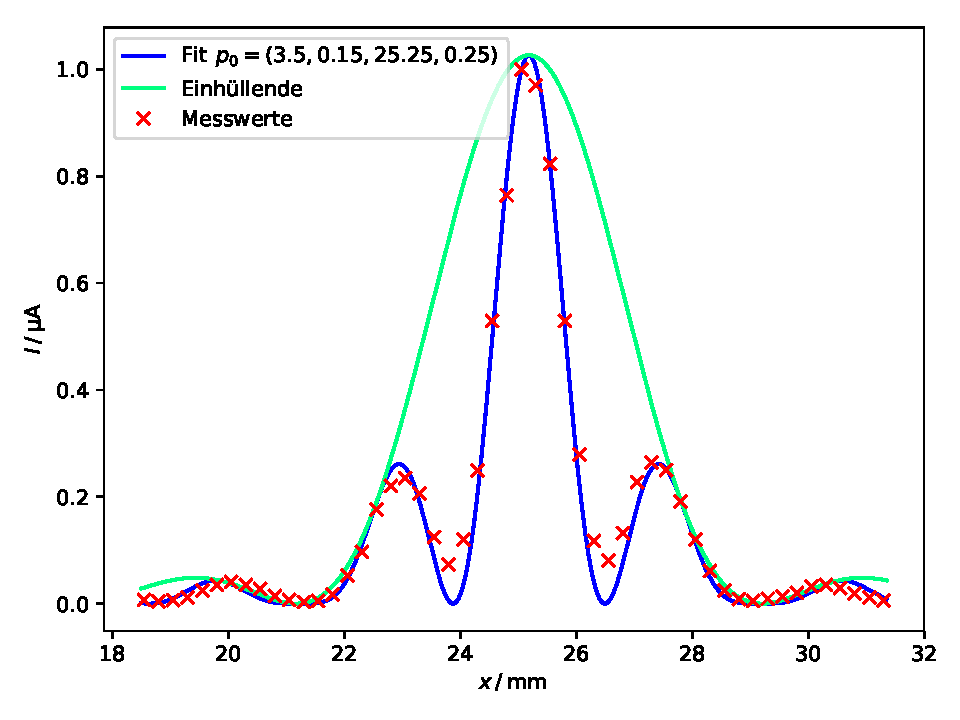
\includegraphics[width=\textwidth]{Plots/1doppel.pdf}
  \caption{Graph zur Bestimmung der Breite und des Abstandes des Doppelspalts mit den Parametern $(A_0, b, x_0, g)$.}
  \label{fig:1dop}
\end{figure}

Eine Regression
\begin{equation*}
  f(x) = A^2_0 b^2 \left(\frac{\lambda}{\pi b \sin{\!\left(\frac{x-x_0}{L} \right)}}\right)^2 \cos^2{\!\left(\frac{\pi g \sin{\!\left(\frac{x-x_0}{L}\right)}}{\lambda} \right)} \sin^2{\!\left(\frac{\pi b \sin{\!\left( \frac{x-x_0}{L}\right)}}{\lambda} \right)}
\end{equation*}
\begin{center}
  \small{($L = \SI{97,5}{\cm}$, $\lambda = \SI{635}{\nm}$)}
\end{center}
liefert die Werte
\begin{align*}
  A_0 &= \SI{6,6(1)}{\uA \per \mm}\\
  b &= \SI{0,154(2)}{\mm}\\
  x_0 &= \SI{25,19(1)}{\mm}\\
  g &= \SI{0,237(3)}{\mm}.
\end{align*}

Die Herstellerangaben betragen $b_\text{theo} = \SI{0,15}{\mm}$ und $g_\text{theo} = \SI{0,25}{\mm}$.
Die gemessene Breite liegt in einem $2 \sigma$-Intervall. Der relative Fehler beträgt $\SI{2,79}{\%}$.
Der gemessene Abstand liegt in einem $5 \sigma$-Intervall und der relative Fehler beträgt $\SI{5,41}{\%}$.

\subsubsection{2. Messung \label{sec:2dop}}

In Tabelle \ref{tab:2dop} befinden sich die aufgenommenen Messwerte.
\begin{table}[H]
   \centering
   \caption{Messwerte zur Bestimmung der Breite und des Abstandes des Doppelspalts}
   \label{tab:2dop}
   \begin{tabular}[t]{ c c }
 \toprule
 {$x\:/\: \mathrm{mm}$} & {$I\:/\: \symup{\mu A}$} \\
    \midrule
    21,6 & 0,038 \\
    21,8 & 0,058 \\
    22,0 & 0,082 \\
    22,2 & 0,100 \\
    22,4 & 0,140 \\
    22,6 & 0,250 \\
    22,8 & 0,500 \\
    23,0 & 0,800 \\
    23,2 & 0,900 \\
    23,4 & 0,850 \\
    23,6 & 0,750 \\
    23,8 & 0,900 \\
    24,0 & 1,500 \\
    24,2 & 2,250 \\
    24,3 & 2,400 \\
    24,4 & 2,500 \\
    24,5 & 2,250 \\
    24,6 & 2,400 \\
    24,7 & 1,750 \\
    24,8 & 1,800 \\
    24,9 & 1,750 \\
    25,0 & 1,600 \\
    25,1 & 2,200 \\
    25,2 & 2,050 \\
    25,3 & 3,000 \\
    25,4 & 2,600 \\
    \bottomrule
  \end{tabular}
  \qquad
  \begin{tabular}[t]{ c c }
\toprule
{$x\:/\: \mathrm{mm}$} & {$I\:/\: \symup{\mu A}$} \\
   \midrule
    25,5 & 3,200 \\
    25,6 & 3,200 \\
    25,8 & 3,200 \\
    25,9 & 2,000 \\
    26,0 & 2,400 \\
    26,1 & 1,500 \\
    26,2 & 1,600 \\
    26,3 & 1,550 \\
    26,4 & 1,700 \\
    26,5 & 1,950 \\
    26,6 & 2,000 \\
    26,7 & 2,200 \\
    26,8 & 2,000 \\
    26,9 & 1,950 \\
    27,0 & 1,600 \\
    27,1 & 1,350 \\
    27,2 & 1,100 \\
    27,4 & 0,650 \\
    27,6 & 0,500 \\
    27,8 & 0,500 \\
    28,0 & 0,500 \\
    28,2 & 0,460 \\
    28,4 & 0,300 \\
    28,6 & 0,175 \\
    28,8 & 0,055 \\
    \bottomrule
  \end{tabular}
\end{table}


Von der Intensität $I$ muss erneut der Dunkelstrom $I_\text{d} = \SI{0,002}{} \: \symup{μA}$ abgezogen werden und die Werte werden erneut normiert.
Die Werte sind in Abbildung \ref{fig:2dop} aufgetragen.
\begin{figure}[H]
  \centering
  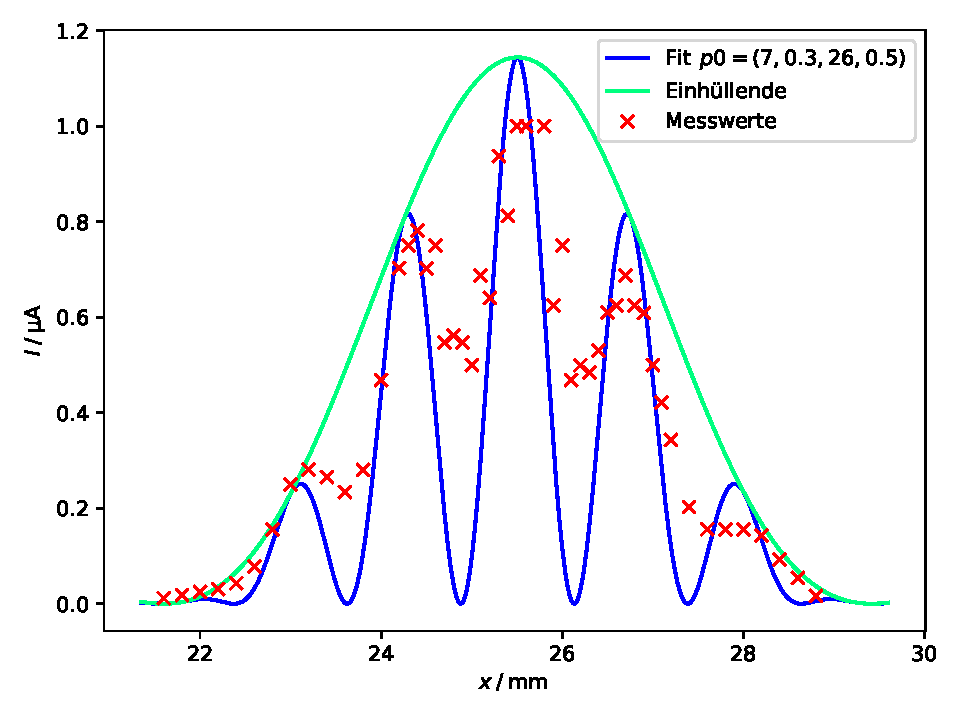
\includegraphics[width=\textwidth]{Plots/2doppel.pdf}
  \caption{Graph zur Bestimmung der Breite und des Abstandes des Doppelspalts mit den Parametern $(A_0, b, x_0, g)$.}
  \label{fig:2dop}
\end{figure}

Die Regression aus Kapitel \ref{sec:1dop} ergibt die Werte
\begin{align*}
  A_0 &= \SI{6,8(4)}{\uA \per \mm}\\
  b &= \SI{0,16(1)}{\mm}\\
  x_0 &= \SI{25,51(2)}{\mm}\\
  g &= \SI{0,494(9)}{\mm}.
\end{align*}

Die Breite weicht mit einem relativen Fehler von $\SI{5,49}{\%}$ von der Herstellerangabe
$b_\text{theo} = \SI{0,15}{\mm}$ ab und liegt dabei in einem $1 \sigma$-Intervall.
Die Herstellerangabe für den Abstand beträgt $g_\text{theo} = \SI{0,5}{\mm}$.
Der gemessene Wert liegt ebenfalls in einem $1 \sigma$-Intervall und der relative Fehler beträgt $\SI{1,25}{\%}$.
